\documentclass[a4paper]{article}

\usepackage[english]{babel}
\usepackage[utf8]{inputenc}
\usepackage{amsmath}
\usepackage{graphicx}
\usepackage[colorinlistoftodos]{todonotes}
\usepackage{float}
\usepackage{url}

\title{The Scrollet}

\author{Matthew Flickner and Joseph Barbosa}

\date{\today}

\begin{document}
\maketitle

\begin{abstract}
Our design, the Scrollet, explores the potential for a touch-based, tablet-style device with a flexible screen that rolls up into itself. The features included make the Scrollet a better version of the computing tablet and the tablet's natural evolution.
\end{abstract}


\section{Introduction}
Historically, a tablet is a chunk of stone of clay that ancient cultures used to write on. They were large, clunky, and hard to carry. In addition, tablets easily cracked and broke.
\begin{figure}[H]
\centering
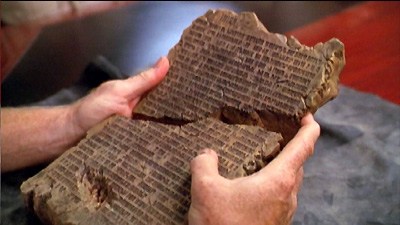
\includegraphics[width=0.5\textwidth]{ancienttablet.jpg}
\end{figure}
Modern day electronic tablets obviously are not nearly as chunky and heavy but many of the characteristics of ancient tablets still hold true to modern day ones. Both ancient and modern tablets are fixed in size and they are not the easiest to carry. And they crack and break very easily, especially when dropped. Yet for some reason, tablets these days are all the rage. Apple iPad, the Google Nexus, the Samsung Galaxy Tab, the Windows Surface are all very popular buys as they aim to find the middle ground between a mobile phone and a laptop. But tablets these days just don't enough. Their design has failed to provide a successful model of a portable device that is the middle ground between a computer and a mobile phone. The tablet's time is done. Ancient tablets were eventually replaced with the far more efficient paper. Paper took on many various forms but one of the most efficient was the scroll. And that is were we come in. It's time to replace the modern day computing tablet with the next step in it's evolution. It is time for the modern computing scroll. The following is our proposed design for a computing scroll, the Scrollet.


\section{Top Level Design}
\begin{figure}[H]
\centering
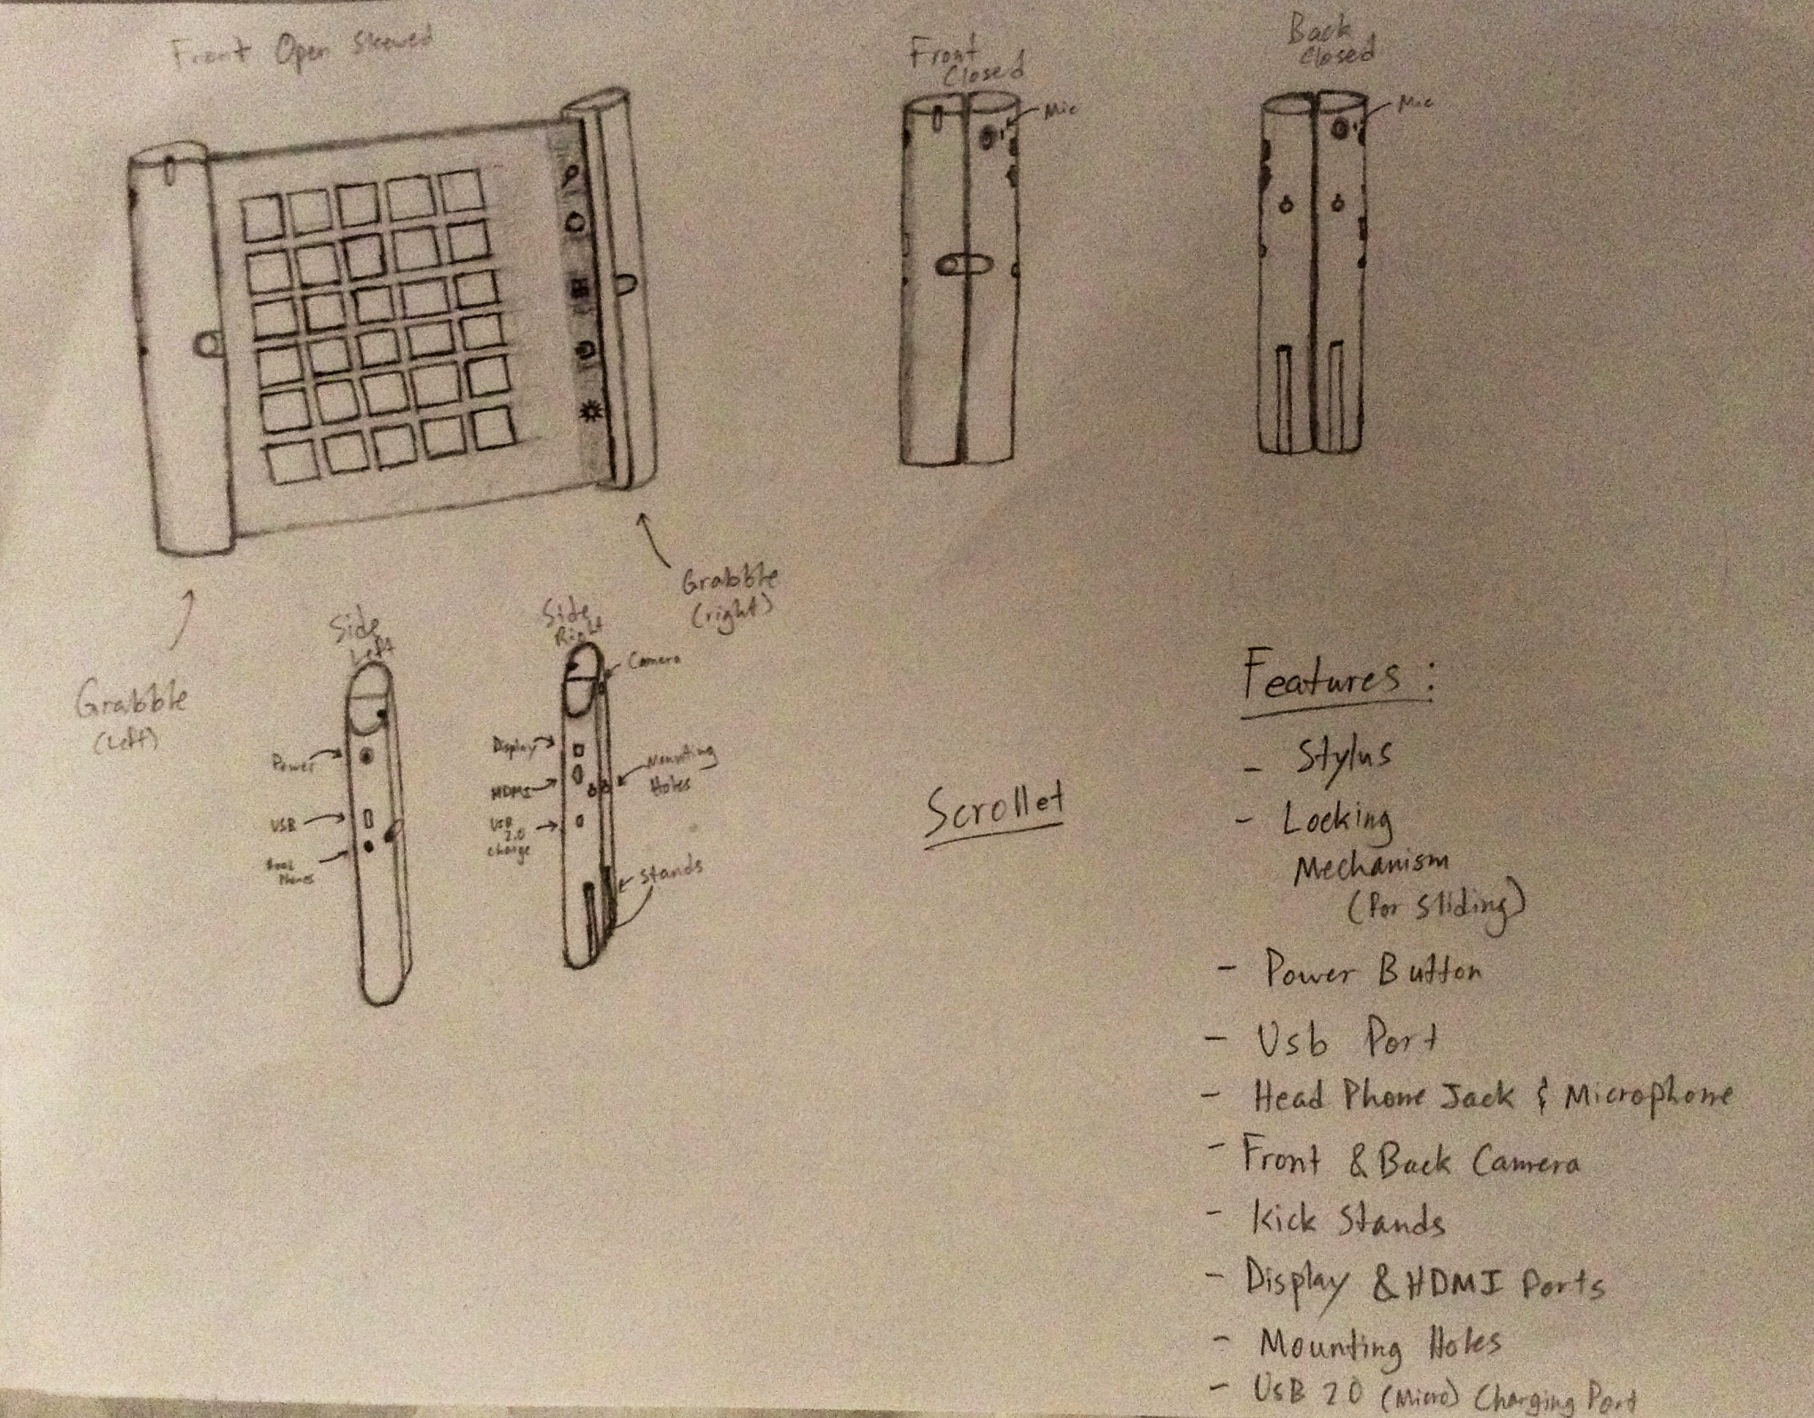
\includegraphics[width=0.8\textwidth]{scrollet-scan.jpeg}
\caption{Overall Conceptual Design for the Scrollet Device}
\end{figure}
\subsection{Hardware Overview}
The Scrollet, naturally, is designed like to work like a scroll. It is similar to the design of the Xpaaand conceptualized by Khalilbeigi but with more features and different usage and implementation of the flexible screen. \cite{Khalilbeigi} It has two "Grabbles" on the sides from which the screen rolls into. When the Scrollet is closed, all that is visible are the two Grabbles. There is a manual push switch that can be used to lock the Scrollet in closed position. Upon pulling the Grabbles apart, a thin, flexible screen comes out. Upon being fully pulled out, a switch will trip and the screen will lock in the out position. The switch is tripped by pulling the screen out to it's maximum length then releasing. To roll the screen back into the Grabbles, the switch is tripped again and will slowly pull the screen in itself with the user guiding it in.

\subsection{The Grabbles}
The Grabbles are where mostly everything occurs in the Scrollet. Their shape is that of a parabolic cylinder. Inside the Grabbles are the processor, memory, storage, graphics card, battery, speakers, accelerometers, compass, GPS, light sensors, WiFi antenna, and Bluetooth chip. In addition, the inside of the grabbles will have some protective cushioning to better protect the screen and other critical components. On the exterior of the Grabbles are the HDMI input, Mini-Display input, headphone port, stylus slot, power button, camera, a USB 3.0 port for additional storage, and a USB Micro port to be used for charging as well as syncing data to computers. On the backside of the Grabbles, there is an adjustable kickstand that can be used to prop up the Scrollet during use, a retractable support beam for hold the device steady for one hand use, and two mounting holes that would allow for the Scrollet to be mounted on a wall.

\subsection{The Screen}
The screen is what makes the Scrollet stand out. It is thin and flexible and has the ability to roll up and roll out. The ability of the screen to do this comes from advances in OLED screens technology.

\subsubsection{Some Information About OLED Displays}
OLED stands for "Organic light-emitting diode" \cite{Lin}. OLED screens are considered to be a promising alternative to modern LCD displays on mobile devices.\cite{Lin} OLED's provide brighter colors, wider viewing angles and image response times. However OLED displays are self-emmisive and therefore power consumption is highly dependent on the image content \cite{Lin}.

\subsubsection{Innovation in OLED's}
The technology made possible for the Scrollet has a lot to with recent developments by LG.
\begin{figure}[H]
\centering
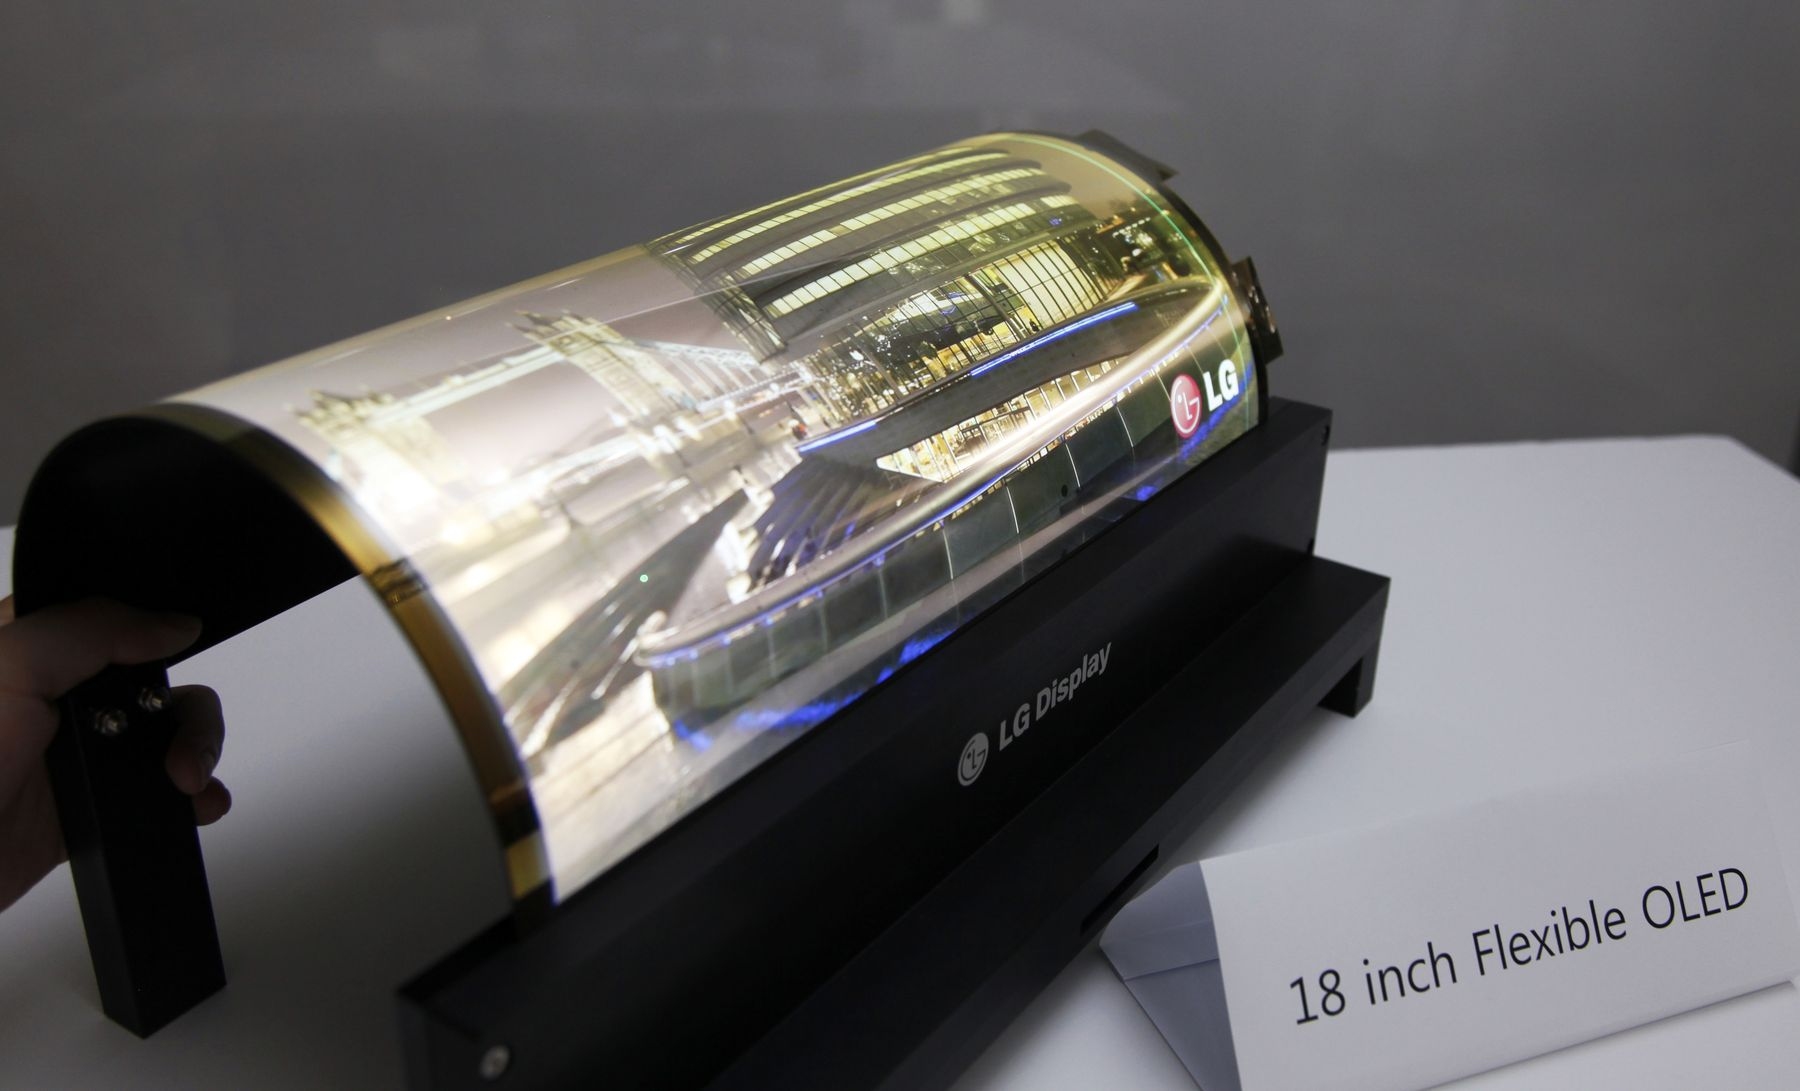
\includegraphics[width=0.5\textwidth]{lgoled.jpg}
\caption{LG's Flexible 18-inch OLED Display.}
\end{figure}
LG Display recently announced their 18-inch flexible OLED panel as well as a 18-inch transparent OLED panel \cite{LG}. The resolution is pretty good, getting a resolution of 1200 x 810  with nearly 1 million mega-pixels \cite{LG}. But more importantly the panel can be rolled up to a radius of 3 cm (diameter of 6 cm) without affecting the functionality of the display \cite{LG}. They achieved flexibility and thinness by making the displays out of a polyimide film instead of conventional plastic \cite{LG}.

\subsubsection{The Screen of the Scrollet}
The Scrollet screen is designed based on this pioneering innovation in displays from LG. The Scrollet combines this new technology with current mobile device touch screen technology and accelerometers to create essentially a working electronic scroll.

\subsection{Software Overview}
The root operating system of the Scrollet is a very simple touch-based operating system that offers very few options to the user. Its main purpose to serve as essentially a boot menu for the virtual guest systems that are run inside the root. That being said the root operating system has essentially 5 main functions.

\subsubsection{DisplayMode}
The first function is to enter DisplayMode. Display Mode allows for the Scrollet to be used as a external monitor for a computer. This can be done through the HDMI or MiniDisplay port as well as over Wi-Fi similarly to Apple AirPlay.

\subsubsection{MainMode}
MainMode is where most of the Scrollet's user usage will occur. Essentially MainMode is a virtual machine that allows for the user to run another operating system as a guest system on top of the root operating system. Users will obviously only be able to use guest operating systems that support touch interface. The 3 operating systems currently that would be considered able to be used on Scrollet are Windows 8.1, Android OS for tablets, and iOS for tablets. They would use virtual hard disks for storage similar to Virtualbox.

\subsubsection{CameraMode}
CameraMode is a simple function that allows for users to access and use the camera without having to boot up into a virtual operating system.

\subsubsection{MusicPlayer}
The music player allows for the user to access and play their music library without having to boot into a virtual system to have their music at their fingertips.

\subsubsection{Settings}
The final function on the root operating system is Settings. Settings is, naturally, where all of the settings for the Scrollet can be accessed. Here users can modify the settings for any virtual operating system they are running and access other device settings.

\subsubsection{Future Software Development}
Eventually Scrollet will develop a more in-depth root operating system similar to that of Android and iOS optimized for the scrollet. However Scrollet will always support the virtualization of any tablet-based operating system of the user's choosing. This is to give the user the option to run the touch-based operating system of their choice.

\section{The System of Use}
The Scrollet is designed to be that middle ground that tablets just never could be. Compressible, efficient, flexible and multifaceted the Scrollet can be used for anything. It can stand upright on by itself, hang from a wall, or tilt at an angle with a kickstand. It can run any touch based operating system. It has stylus and bluetooth keyboard capability. In addition it has everything a tablet has such as front and rear-facing cameras, USB port, speakers, accelerometers and more. The innovation comes with the flexible screen that rolls up into the sides of the scrolls.

\subsection{Potential Usability Issues}
There is no such thing as a perfect product and the Scrollet definitely has some usability issues.
\subsubsection{The Thinness of the Screen}
The biggest of these concerns is how a user touch input would work on such a thin, flexible screen. Normal touch input could force the screen to give way. \cite{Dijkstra} The screen could also bend just as the user is holding it. Screen stability and integrity are a huge concern. Just because the screen is flexible does not mean it is unbreakable. The screen could very easily potentially rip or tear with enough force \cite{Dijkstra}. This is a very important issue which we tried to address in our design. Instead of giving the user manual sizing control of their screen, our screen is design to naturally be pulled taught by the rollers within the Grabbles. The screen then locks in the unrolled position at fixed sizes. This keeps the screen more taunt and hopefully will better allow for the maintaining of tension with touch input. The screen is also surrounded on the top and bottom by a small frame of material that is slightly stronger and less flexible material. This frame also helps with tension and preventing unwanted folds in the screen upon touch. Another issue that comes with the thinness of the screen is how easily the screen will rip. The design with the frame projecting the top and bottom of the screen are intended to prevent this from occurring. 

\subsubsection{Battery Life}
Another usability issue is battery life. The Scrollet is a powerful device and it is uncertain how long it will last when portable. Since OLED's are self-emissive, their power consumption is totally dependent on the image on the screen \cite{Lin}. A black image uses almost no power but a white image could use more than twice the power of an LCD display would use in a normal situation \cite{Lin}. Lin has explored this problem in his studies and developed an algorithm that investigates images based on human visual attention regions to visually break up an image based on those visual attention regions and save energy by using less power to lighting the regions with less visual attention \cite{Lin}. Ideally, power would not be a concern but until then Scrollet would utilize similar method to conserve battery life.

\subsubsection{On-the-Go Usage}
Perhaps the biggest potential issue with the Scrollet is the when using the Scrollet on the go and needing to touch the screen with one handle by removing one hand from one of the Grabbles. With a bendable screen, the Scrollet will, thanks to gravity, bend downwards towards the ground. The best way to counter this effect is by the addition of a retractable support beam that runs behind the screen from Grabble to Grabble which the user would use to support the screen when using Scrollet on the go.

\section{Usage Scenarios}
\subsection{As A External Monitor}
One of the main functions the Scrollet is that it can be used as a portable external monitor. With both wireless and wired ability to be used as a second monitor, the user would be able to bring their Scrollet wherever they go and have a second monitor to use their their laptop if they wished. This is made possible by the Scrollet's ability to stand upright on its Grapples. In addition, wall mounts make the Scrollet easily hung on the wall to further its ability to act as a display.

\subsection{As Computing Tablet-Style Device}
The Scrollet works very well as tablet-style mobile device. It was designed to be the evolution of the tablet so it naturally fits the usage of a tablet. Its roll-up screen ability allows for it to be stored easily and not take up much space. It supports both horizontal and vertical alignment with the Grabbles. It has a touch interface, a camera, wireless, and bluetooth with potential for a bluetooth keyboard. It is essentially is a tablet with a screen that rolls up.

\subsection{New Interaction Techniques}
\subsubsection{Rolled and Unrolled}
Modern day tablets have a power button that is used to both turn the device on and off and put the device in standby. In the Scrollet there is a button for these two functions. However, with a rollable screen, a new method of interaction would allow for the user to put the Scrollet in standby and shut of the screen by rolling up the screen into the Grabbles and powering the screen back on by unrolling the screen out of the Grabbles.
\begin{figure}[H]
\centering
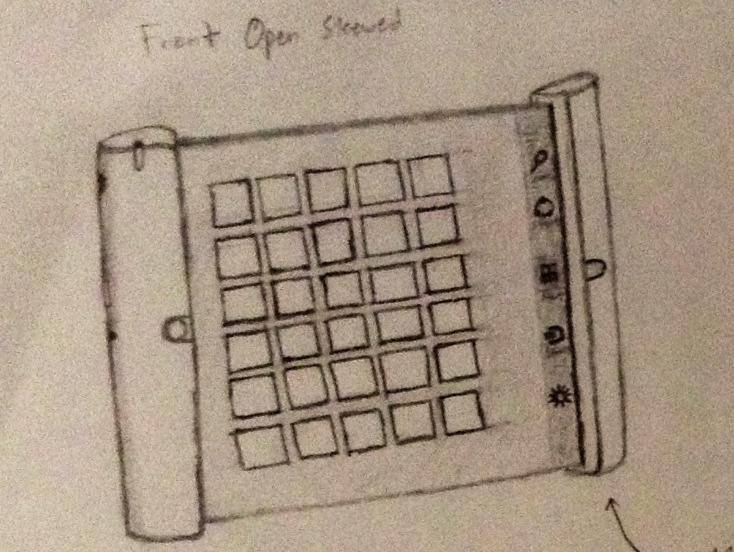
\includegraphics[width=0.4\textwidth]{scrolletopen.jpg}
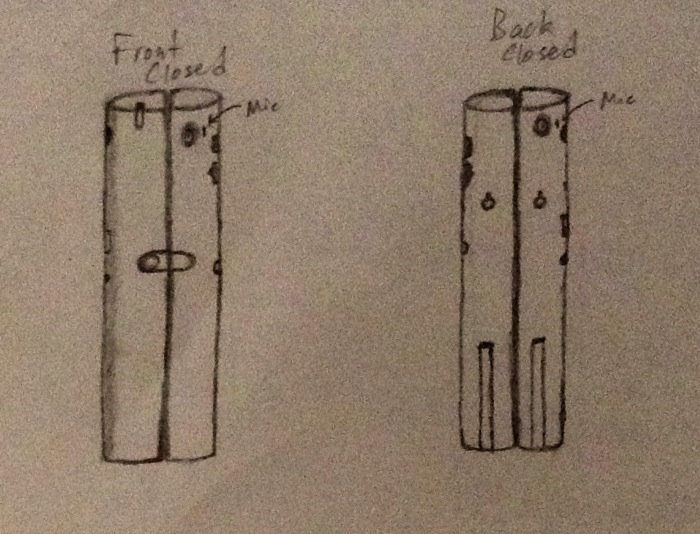
\includegraphics[width=0.4\textwidth]{scrolletclosed.jpg}
\caption{The Scrollet in an open position with screen on and Scrollet closed with screen off.}
\end{figure}

\subsubsection{The Wave Motion}
Another potential interaction technique is made possible through the use of the flexible screen and the accelerometers. Gripping the two Grabbles, the user would be able to use harmonic motion as a way to interact with the Scrollet. This could be one method of scrolling or changing windows in a similar way to swiping left or right on the main menu of a smartphone or table.
\begin{figure}[H]
\centering
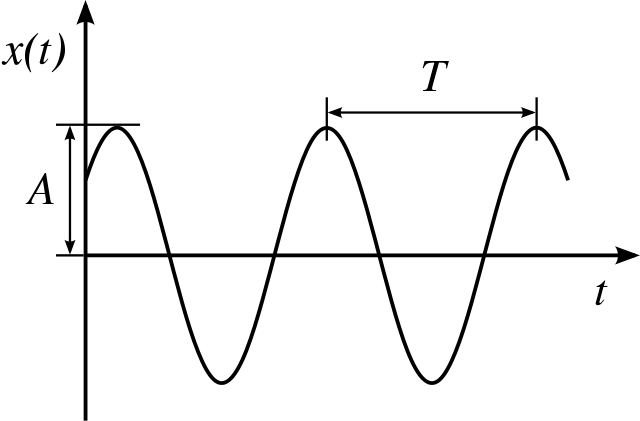
\includegraphics[width=0.4\textwidth]{harmonicwave.png}
\caption{A harmonic wave motion could easily be used to interact with the Scrollet.}
\end{figure}


\section{Why Scrollet is How It Is - Balance}
\subsection{Universal Usability}
Our goal with the Scrollet was to provide a design that the user for literally anything. This is part of the reason why we implemented virtualization of touch based operating systems. We wanted the user to be able to choose the operating system of their preference and go with it. This is also why the Scrollet can be used as a external monitor as well as a tablet-style device. We want the Scrollet to be able to be used in all scenarios \cite{Nielsen}. This is also why we included a stylus, to allow the user to decide whether they wished to use their fingers for the touch implementation or to use the stylus for writing. This is why we allow for a bluetooth keyboard for typing. Giving the user the option to use the Scrollet in as many ways as possible for as many things as possible was on of our main priorities.

\subsection{Learnability}
With the Scrollet we wanted our users to learn how to use it very quickly and easily. That is why we modeled it very closely after tablets, especially as far as user interface goes with a touch-based system. The only really learning that will come with the Scrollet will be the user's getting used to the virtualization touch-based operating systems. With a proper tutorial in the software, the user will be able to easily learn how to run these guest systems as they please. But with a device such as this, it is better to have more usability than learnability, so a bit of a learning curve with regards to the virtualization is a good thing because the users will get far more usability out of the Scrollet \cite{Tog}. We want to make the device relatively learnable but balance that out with maximizing as much usability as we can.


\section{Usability Metric Analysis}
\subsection{Learnability}
We expect the Scrollet to excel well in the learnability category because we have modeled it so close to a tablet. Since, the Scrollet is used like a tablet, the learnability overall with not be too difficult despite its new features and methods of interaction. Although not that weak of a category, learnability is still most likely to be the Scrollet's weakest category due to the different physical design.
\subsection{Efficiency}
Efficiency is what the Scrollet was designed for. It is supposed to be the universal device that you can take anywhere and do anything with. It integrates features from displays, tablets, and computers to combine into one device for it all. It is customizable to the user's experience which further improves the level of efficiency that the user can achieve from the Scrollet.
\subsection{Errors}
Errors are hard to estimate with a conceptual designed but there are sure to be some user errors with the Scrollet. Potential errors would most likely stem from the user not being used to the thin screen or not being used to how the roll up screen. With the not too difficult learnability of the Scrollet, the user should quickly eliminate errors and be able to use the Scrollet with maximum efficiency.
\subsection{Satisfaction}
Satisfaction is what we hope is our highest ranking. Everything that the Scrollet allows for efficiently should combine with it's easy learnability (for the most part) and make the user incredibly satisfied with the product they are getting. 

\section{Conclusion}
Overall, the Scrollet has the potential to be the device of the future. It is designed to be the one-for-all, end-all device that does everything and can still be stored in a small compact space and taken anywhere. Just like the scroll and paper eventually replaced the ancient table, it is now time for the Scrollet to replace the modern computing tablet. Scrollet is just simply the the next step in the evolution of mobile computing.

\bibliography{references}
\bibliographystyle{plain}


\end{document}